\documentclass[a4paper]{article}
\usepackage[utf8]{inputenc}
\usepackage[spanish]{babel}
\usepackage{titlesec}
\usepackage{mathptmx} % Fuente Times New Roman
\usepackage{graphicx}

% Interlineado
\usepackage{setspace}
\onehalfspacing

% Tamaño de fuente para secciones
\usepackage{sectsty}
\sectionfont{\fontsize{16}{15}\selectfont}
\subsectionfont{\fontsize{14}{15}\selectfont}
\subsubsectionfont{\fontsize{12}{15}\selectfont}

% Especiado anterior y posterior
\titlespacing*{\section}{0pt}{0pt}{0pt}
\titlespacing*{\subsection}{0pt}{0pt}{0pt}

% Header y footer
\usepackage{fancyhdr}
\pagestyle{fancy}
\fancyhead{}
\fancyhead[C]{Análisis de Técnicas de IA para videojuegos en Unity}
\fancyfoot{}
\fancyfoot[L]{Nahuel Castro, Melina Lazzaro, Agustín Pérez Leiras, Sebastián Rial}
\fancyfoot[R]{\thepage}
\renewcommand{\headrulewidth}{0pt}
\renewcommand{\footrulewidth}{0pt}

\begin{document}

\begin{titlepage}

    \title{
        \textbf{Análisis de Técnicas de IA para \\ videojuegos en Unity} \\[2.5ex]
    }

    \author{
        \textbf{Tutor:} Hernán Merlino \\[2.5ex]
        \textbf{Alumnos} \\[2.5ex]
        Nahuel Castro, \textit{(Padrón \# 106.551)} \\ \texttt{ ncastro@fi.uba.ar } \\[2.5ex]
        Melina Lazzaro, \textit{(Padrón \# 105.931)} \\ \texttt{ mlazzaro@fi.uba.ar } \\[2.5ex]
        Agustín Pérez Leiras, \textit{(Padrón \# 100.972)} \\ \texttt{ aperez@fi.uba.ar } \\[2.5ex]
        Sebastián Rial, \textit{(Padrón \# 90.309)} \\  \texttt{ riseba@gmail.com } \\[2.5ex]
        \\[2.5ex]
        \normalsize{Facultad de Ingeniería, Universidad de Buenos Aires} \\
    }

    \date{21 Nov 2023}

\end{titlepage}

\maketitle

\newpage

\begin{abstract}

    Este trabajo consistirá en primera instancia en la investigación y exploración del estado del arte de las técnicas de inteligencia artificial utilizadas en el desarrollo de videojuegos en Unity, para luego desarrollar y ampliar sobre las capacidades existentes. En específico, trabajaremos con algoritmos de toma de decisiones, pathfinding y reinforcement learning aplicadas a un videojuego sencillo donde un jugador compite contra personajes controlados por inteligencia artificial.\\

    Initially, this project consists of researching and exploring the state of the art in artificial intelligence techniques used in the development of videogames in Unity, followed by the development and enhancement of existing capabilities. Specifically, we focused on decision-making algorithms, pathfinding, and reinforcement learning applied to a simple videogame where a player competes against characters controlled by artificial intelligence.

\end{abstract}

\section{Palabras clave / Keywords}

Videojuegos, Videogames, Inteligencia Artificial, Artificial Intelligence, Unity, Pathfinding, Algoritmos de toma de decisión, Decision-Making Algorithms, Machine Learning, Reinforcement Learning.

\section{Introducción}

\subsection{Inteligencia artificial en videojuegos}

En los últimos años se ha visto un avance acelerado en el campo de la inteligencia artificial (IA) en diversos campos como medicina, industria automotriz, procesamiento de datos, toma de decisiones, traductores, videojuegos, entre otros. Este proyecto se centrará en la aplicación de IA en el sector de los videojuegos.

La implementación de IA en los videojuegos difiere con respecto a otros campos, fundamentalmente por la naturaleza de los mismos, que constan de múltiples procesos ejecutándose en simultáneo en tiempo real, como la renderización de gráficos o la simulación de físicas, por lo que la IA debe estar diseñada de manera eficiente ya que debe compartir recursos con estos procesos. Además, el enfoque principal en este caso no radica en modelar los distintos componentes del juego de forma extremadamente realista o inteligente, sino en lograr que estos componentes reaccionen a las acciones del jugador o eventos del juego de una forma que tenga sentido y contribuyan a crear una experiencia más entretenida o inmersiva; por lo que muchos de los algoritmos comúnmente utilizados en los videojuegos tienden a ser más sencillos.

Se puede hacer una distinción principal entre las formas en las que la IA puede aplicarse en el contexto de los videojuegos. Por un lado, se puede emplear de forma generativa, asistiendo a los desarrolladores en el proceso de creación de escenarios, personajes, diálogos, entre otros. Por el otro, la IA puede operar en tiempo real dentro del videojuego, otorgando la impresión de que distintos elementos del mismo actúan de manera inteligente, proporcionando experiencias únicas en cada partida que logran prolongar el interés de los jugadores. En este proyecto nos vamos a centrar en el segundo uso.

Esto puede tomar distintas formas, desde comportamientos variados en personajes no jugables (o \textit{NPCs}, por sus siglas en inglés Non Player Characters) que interactúan con el jugador, hasta algoritmos que detectan el nivel de habilidad del jugador para ofrecer una dificultad adaptativa, de forma que el jugador siempre tenga enfrente un desafío acorde a su nivel de habilidad, evitando que se aburra por ser muy fácil o se frustre por ser muy difícil.

\subsection{Motores de videojuegos}

El desarrollo de un videojuego desde cero puede resultar sumamente desafiante, en parte debido a la complejidad técnica de tareas comunes como la gestión de gráficos, físicas, recursos, entre otros. Para simplificar este proceso existen herramientas denominadas motores de videojuegos, que proporcionan una base sólida con varios de esos sistemas comunes predefinidos, permitiendo a los desarrolladores centrarse en los aspectos particulares de su juego.

Entre los motores más populares se encuentran \textit{Unity} y \textit{Unreal Engine}. A continuación, profundizaremos en las características de cada uno.

\textbf{Unity}: es una herramienta muy versátil y ampliamente utilizada, lo que presenta la ventaja de contar con una extensa documentación, abundante material de referencia y aprendizaje, así como también una comunidad muy activa. El material disponible, la estructura del editor y el hecho de que utiliza C\# como lenguaje de programación para los scripts facilitan su adopción y reducen su curva de aprendizaje.

\textbf{Unreal Engine}: destaca principalmente por su potencia gráfica, que permite la creación de mundos extremadamente realistas. Utiliza C++ como lenguaje de programación pero además ofrece una herramienta más sencilla y visual de realizar los scripts mediante los denominados Blueprints.
Sin embargo, presenta una curva de aprendizaje más pronunciada que la de Unity, requiriendo una inversión de tiempo mayor para aprovechar al máximo sus capacidades.

Para el desarrollo de este proyecto, como el foco está en la implementación de modelos de IA y no en la creación de un videojuego con una alta calidad gráfica, optamos por utilizar Unity puesto que no se justifica superar la curva de aprendizaje de Unreal Engine si no vamos a hacer uso de sus capacidades gráficas avanzadas.

Este proyecto se centrará en explorar las distintas herramientas que ofrece Unity para la implementación de IA y demostrar su aplicabilidad a través de la creación de un videojuego simple que muestre estos modelos en acción. En la sección Estado del Arte de este documento ahondamos en detalle en el estado del arte de la IA en Unity y en la secciones de Problema Detectado y Solución Propuesta, qué espacio de mejora e innovación detectamos y cómo llenar este espacio.

\section{Estado del Arte}

A continuación, profundizaremos en las técnicas más populares para implementar IA en videojuegos en la actualidad, algunas de las cuales serán utilizadas para la implementación del presente trabajo.

\subsection{Algoritmos de toma de decisiones}

Son procedimientos lógicos utilizados para seleccionar la mejor opción entre varias posibles en función de ciertos criterios. Para el caso de los videojuegos, son la base de todo el comportamiento de los agentes.

\subsubsection{Máquinas de Estado Finito}

Una máquina de estado finito (FSM, por sus siglas en inglés Finite State Machine), también conocida como autómata finito, es un dispositivo que contiene un número finito de estados, de los cuales solo uno puede estar activo a la vez. Se parte de un estado inicial y diversos eventos del juego pueden disparar transiciones de un estado a otro. Es una de las formas más sencillas e intuitivas de modelar el comportamiento de un agente, además de tener poco \textit{overhead} de procesamiento \cite{programming_game_ai_by_example}, lo que lo convierte en una técnica ampliamente utilizada, siendo incluso la única técnica de IA utilizada en muchos videojuegos \cite{unity_artificial_intelligence_programming}. Sin embargo, presenta la dificultad de que la cantidad de estados aumenta de forma exponencial al agregar nuevas condiciones, lo que lo hace menos adecuado cuando se tiene una gran cantidad de estados y transiciones.

Un ejemplo emblemático de este tipo de inteligencia artificial son los fantasmas del juego original \textit{Pac-Man}. Estos son autómatas, los cuales tienen una cantidad reducida de estados, para los casos en que tienen que perseguir o escapar del jugador.

Las limitaciones de las FSMs se pueden mitigar parcialmente colocando las FSM dentro de otras FSM, lo que se conoce como \textit{Hierarchical FSMs}. Esto permite contener el aumento en la cantidad de transiciones necesarias \cite{finite_state_machine_in_game_development}.

En \textit{Unity} se pueden encontrar múltiples librerías para facilitar el diseño de una IA basada en autómatas. [\textit{Playmaker}, \textit{Bolt}, \textit{Animator Controller}, \textit{State Machine}].

\begin{figure}[ht]
    \centering
    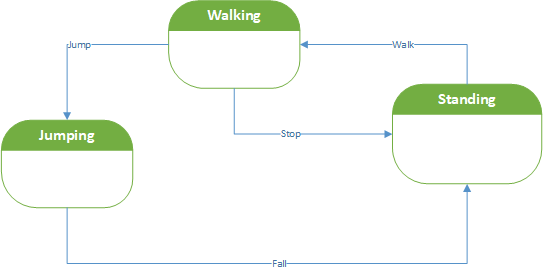
\includegraphics[width=0.8\textwidth]{./images/finite-state-machine.png}
    \caption{Diagrama de una maquina de estados finitos para el movimiento de un agente}
    \label{fig:fsm}
\end{figure}

\subsubsection{Árboles de Comportamiento}

Los árboles de comportamiento son estructuras jerárquicas (grafos dirigidos acíclicos con raíz) donde los nodos internos son llamados nodos de control de flujo y los nodos hoja son llamados nodos de ejecución \cite{behavior_tress_in_robotics_and_ai}. Los nodos de control de flujo son los encargados de determinar si se deben ejecutar o no sus nodos hijos. Modelar el comportamiento de agentes de esta forma permite que la lógica surja de recorrer el árbol ejecutando los nodos indicados. Los árboles de comportamiento ofrecen una mejor escalabilidad que las máquinas de estado finitas, ya que las relaciones jerárquicas entre nodos reducen las interacciones a aquellos que comparten un nodo padre, facilitando la gestión de comportamientos complejos \cite{behavior_tress_in_robotics_and_ai}. Son similares a las máquinas de estado finitas jerárquicas mencionadas anteriormente, pero por lo general son más intuitivos de implementar que estas últimas.

Uno de los primeros juegos que popularizó esta técnica fue \textit{Halo 2}, que presenta una amplia  variedad de enemigos con diversos comportamientos, para lo cual los árboles de comportamiento demostraron ser una opción altamente efectiva \cite{implementation_of_behavior_tree_in_halo_2}, mientras que las FSMs habrían supuesto un verdadero desafío de mantenimiento.

En \textit{Unity} existen múltiples herramientas para el diseño de IAs basadas en árboles de comportamiento. La mayoría de estas herramientas permiten diseñar árboles de comportamiento en forma visual para hacer más intuitivo su desarrollo [\textit{Behaviour Designer}, \textit{Emerald AI}, \textit{RAIN AI}, \textit{uNode}]. Utilizaremos este tipo de algoritmos para la implementación de IA basada en algoritmos tradicionales.

\begin{figure}[ht]
    \centering
    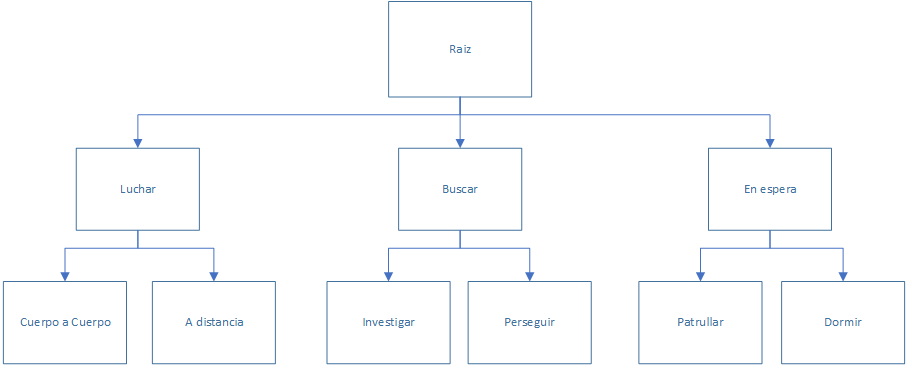
\includegraphics[width=1\textwidth]{./images/behaviour-tree.png}
    \caption{Arbol de decision simple para el comportamiento de un NPC}
    \label{fig:bt}
\end{figure}

\subsubsection{Aprendizaje automático (Machine Learning)}

Las bases del aprendizaje automatizado existen desde hace décadas, pero han ganado gran popularidad recientemente. Posiblemente esto se deba al aumento en el poder de procesamiento y en la cantidad de datos disponibles, que potencian las capacidades de las IAs entrenadas por aprendizaje automatizado. Aún así, el entrenamiento de IAs basadas en aprendizaje automático sigue siendo computacionalmente muy costoso para utilizarse como IA de juegos. La mayoría de los usos de aprendizaje automatizado para la IA de videojuegos ha sido en forma de \textit{offline-learning}, que refiere al entrenamiento de IAs durante la etapa de desarrollo del juego, y no durante el transcurso del juego mismo \cite{machine_learning_in_digital_games:_a_survey}.

A su vez, tiene otras desventajas, a saber:

El resultado de entrenar un agente con aprendizaje automático puede verse como una "caja negra". Es difícil o imposible obtener información sobre su comportamiento esperado a partir de analizar la red neuronal resultante \cite{deep_learning_black_box_problem}.

Son difíciles de entrenar en forma genérica. Incrementar la capacidad de cómputo utilizada mejora permite obtener mejores resultados, sin embargo, hacerlo de forma simplista tiene una alta probabilidad de caer en “overfitting”, IAs que solo logran un objetivo bajo condiciones muy específicas, y cuya performance se degrada en considerablemente al variar ligeramente las condiciones \cite{an_evaluation_of_the_unity_machine_learning_agents_toolkit}.

A pesar de estas desventajas, se ha demostrado que este tipo de entrenamiento de IA tiene una gran capacidad para entrenar agentes altamente capaces, con comportamientos que resultan más "reales" que aquellos logrados utilizando las técnicas tradicionales de IA para videojuegos \cite{a_study_on_overfitting_in_deep_reinforcement_learning}. Por este motivo, vale la pena explorar las posibilidades que presenta el uso de machine learning para el modelado de IAs.

Algunos ejemplos de esto son el juego “Dota 2”, en el cual se utilizaron una serie de técnicas de “reinforcement learning” para entrenar una IA que puede manejar los 5 jugadores de un equipo. Esta IA fue capaz de vencer al equipo campeón en el campeonato mundial del año 2019, en un juego altamente complejo y competitivo \cite{dota_2_with_large_scale_deep_reinforcement_learning}. Otro ejemplo es el de \textit{Alpha Zero}, IA que \textit{Google} entrenó para jugar al Ajedrez, logrando vencer a la mejor IA existente hasta ese momento, \textit{Deepfish}, la cual fue desarrollada con otras técnicas de IA \cite{ai_in_human-computer_gaming}.

Para \textit{Unity} existe el set de herramientas \textit{ML-Agents}, el cual se basa en \textit{PyTorch} para brindar la posibilidad de aplicar diferentes algoritmos de aprendizaje automático sobre modelos generados con el motor de \textit{Unity}. Esos modelos pueden ser luego utilizados para los agentes dentro del juego \cite{an_evaluation_of_the_unity_machine_learning_agents_toolkit}. Algunos de estos algoritmos serán utilizados en el presente trabajo para la implementación de la IA basada en Machine Learning.

\begin{figure}[ht]
    \centering
    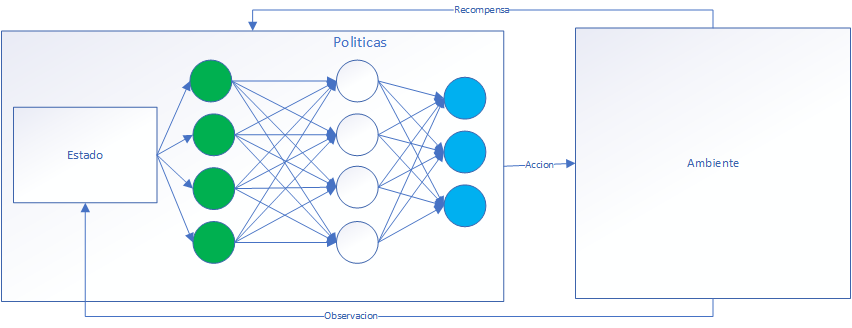
\includegraphics[width=1\textwidth]{./images/deep-learning.png}
    \caption{Método genérico de entrenamiento por red neuronal}
    \label{fig:ml}
\end{figure}


\subsection{Algoritmos de Pathfinding}

Una de las problemáticas más comunes a la hora de desarrollar un videojuego es la necesidad de encontrar caminos a través del escenario del juego, lo cual se conoce como Pathfinding. Por ejemplo, para determinar la trayectoria que sigue un enemigo que se desplaza por el escenario persiguiendo al jugador y esquivando obstáculos. Este es uno de los usos más clásicos de la IA en videojuegos por lo que existen múltiples algoritmos para resolver esta problemática, entre los más utilizados se encuentran \textit{A*}, \textit{Dijikstra}, o \textit{BFS} (Breadth-First Search). Al tratarse de algo tan recurrente existen además una variedad de algoritmos para comportamientos particulares, como PSO (\textit{Particle Swarm Optimization}) el cual permite que un conjunto de agentes se muevan en forma coordinada.

Estos algoritmos se pueden complementar con técnicas para representar eficientemente el espacio como la \textit{Navigation Mesh}, para lo cual Unity provee una serie de herramientas en su módulo de NavMesh \cite{unity_artificial_intelligence_programming}.

En este trabajo utilizaremos algunos de estos algoritmos, a definir basándose en cual sea el más conveniente para cada caso.

\subsection{Otros algoritmos de interes}

Hay una importante cantidad de algoritmos que pueden considerarse de toma de decisiones, pero que apuntan a resolver una funcionalidad muy específica. Existen algoritmos para animación (Inverse Kinematics), toma de decisiones tácticas (Monte Carlo Tree Search, Rule-based Systems), modelado de oponentes (Case-Based reasoning, Redes Bayesianas) y muchos otros. La utilización de estos será definida durante el transcurso del proyecto.

\section{Problema detectado y/o faltante}

Existe una necesidad constante de mejorar la IA en los videojuegos por varias razones:

\begin{itemize}
    \item \textbf{Realismo}: La IA debe dar al usuario la “ilusión de inteligencia” \cite{programming_game_ai_by_example}\cite{unity_artificial_intelligence_programming}. La detección de deficiencias en la lógica de la IA por parte de los jugadores puede disminuir la calidad de la experiencia de juego, reduciendo la inmersión de los jugadores, lo que resulta en un juego menos entretenido \cite{programming_game_ai_by_example}. A su vez,  a menudo, estas deficiencias se intentan compensar otorgando ventajas a los agentes no jugadores, pero este tipo de equilibrio suele parecer injusto para los jugadores, que ven cómo la IA está “haciendo trampas”, lo que degrada también la calidad de la experiencia para el usuario \cite{programming_game_ai_by_example}. Por ello, es relevante explorar las técnicas disponibles para modelar una IA que ofrezca tanto desafío como inmersión y equilibrio al jugador.
    \item \textbf{Entretenimiento y desafío para el jugador}: Si los NPCs pueden dar un nivel de desafío adecuado a la habilidad del jugador, esto resultará en una experiencia más atrapante \cite{artificial_intelligence_for_video_game_visualization}.
    \item \textbf{No repetitividad}:  Si se encuentra una estrategia para la cual es fácil ganarle a la IA, el juego se torna aburrido y simple, es por esto que las IAs deben apartarse a las diferentes estrategias para permitir que la rejugabilidad y que el jugador experimente con diferentes posibilidades.
    \item \textbf{Posibilidad de aprendizaje}: Se pueden implementar IAs que logren aprender y adaptarse a las acciones del jugador, haciendo más dinámica la jugabilidad, lo que incrementa la longevidad del juego \cite{an_adaptive_game_ai_architecture}\cite{artificial_intelligence_for_video_game_visualization}.
\end{itemize}

En vista de los avances tanto en la complejidad de los videojuegos en sí, como así también en las capacidades de aprendizaje automatizado y las técnicas utilizadas para ello, creemos que existe una oportunidad para mejorar todos estos aspectos utilizando técnicas modernas de IA.

\section{Solucion propuesta}

En este trabajo nos proponemos crear un juego en que el jugador compite con otros personajes no jugadores. La idea principal consiste en implementar, para los personajes que compiten con el jugador, dos tipos de comportamiento, uno basado principalmente en algoritmos tradicionales de IA (FSMs, BTs y similares) y otro basado en machine learning (\textit{Reinforcement Learning}, \textit{Imitation learning}, redes neuronales y similares). Es de interés poder, en un estadío final, comparar la performance de ambos tipos de personajes, compitiendo tanto con jugadores como entre sí, y sacar conclusiones al respecto.

A su vez, habrá agentes que utilicen una IA básica, los cuales son adversarios de todos los personajes, y su objetivo principal es ser la fuente de progreso de los jugadores.

\begin{itemize}
    \item Modelado de IA para agentes utilizando técnicas tradicionales (FSMs, BTs, Algoritmos de Pathfinding, CFR, PSO)
    \item Modelado de IA para agentes utilizando técnicas de Reinforcement Learning y Neural Networks (PPO, SAC, MA-POCA, Self-play)
\end{itemize}

En cualquiera de los dos modelos podrán ser utilizados otros algoritmos que complementen la funcionalidad. Por ejemplo, podría haber un agente que utilice \textit{Machine Learning} para ciertas partes de su comportamiento, y algoritmos tradicionales para otra.

\section{Experimentación y/o validación}

El objetivo final es poder comparar la implementación de IA para juegos basada en algoritmos tradicionales, con la implementación basada en aprendizaje automatizado. Esta comparación se puede realizar en múltiples aspectos, a saber:

\begin{itemize}
    \item Facilidad de implementación
    \item Habilidad de juego
    \item Realismo
    \item Predictibilidad
\end{itemize}

A su vez, resulta de interés clasificar los algoritmos según su conveniencia para cada caso de uso, y en qué casos es posible combinarlos para obtener buenos resultados. De esta forma se podrá demostrar que la combinación particular de algoritmos elegidos logra modelar una IA aceptable para el usuario.

El presente trabajo sera públicado en un congreso con referato, mediante la presentación de un \textit{paper}, para la revisión entre pares.

\section{Plan de actividades}

En esta sección establecemos la metodología de trabajo y gestión de proyecto:

\begin{itemize}
    \item \textbf{Metodología}: La metodología a utilizar será una implementación simplificada de Scrum. Se prescinde de ciertos elementos como los roles o las retrospectivas.
    \item \textbf{Herramienta de gestión de proyecto}: Utilizaremos GitHub “Projects”, una herramienta que es parte de GitHub y permite gestionar los principales elementos del proyecto como el backlog de tareas y los milestones.
    \item \textbf{Estimaciones}: Serán realizadas por planning poker. Los “Story Points” representarán la dificultad de la tarea en cuestión, y seguirán la serie Fibonacci.
    \item \textbf{Sprints}: La duración de los Sprints será de 2 semanas. Se realizará una “Sprint Review” a la finalización de cada sprint.
    \item \textbf{Standup Meetings}: Serán realizadas al menos una vez por semana para discutir avances en el trabajo.
    \item \textbf{Documento de diseño del juego}: Este documento proporciona una visión del concepto, mecánicas y demás elementos del juego.
    \item \textbf{Documentación técnica}: Se incluirá la documentación técnica que sea requerida según la complejidad de cada parte del sistema.
    \item \textbf{Manual de usuario}: Documento donde se indica a los usuarios en qué consiste el videojuego y proporciona instrucciones para instalarlo y jugarlo.
    \item \textbf{Entregables}: Los entregables serán el código fuente del juego más los instaladores o paquetes necesarios para su ejecución. A su vez, en cada entrega se adjuntará un video resaltando las funcionalidades nuevas, en caso de que hayan. Al final del proyecto se entregará además el informe final del trabajo.
    \item \textbf{Testing}: Se incluirán tests unitarios para todos los archivos que sean de lógica del juego (archivos de C\#). Se apuntará a tener una cobertura de código superior al 80\%. Para los tests unitarios se utilizará el Unity Testing Framework.
    \item \textbf{Métricas}: Las métricas a utilizar serán el Velocity report, la cantidad de bugs fuera de sprint, y la predictibilidad (cantidad de stories completadas versus planificadas).
    \item \textbf{Quality Assurance}: Los desarrolladores serán los encargados de realizar tests de calidad en cada Sprint. Los issues encontrados deben ser estimados, y podrán realizarse tanto en el Sprint en curso como en los siguientes, basados en el impacto del issue en cuestión.
    \item \textbf{Riesgos}: Los potenciales riesgos que surjan durante el proyecto serán controlados mediante la \textit{Planilla de Definicion de Riesgos} y la \textit{Planilla de Control de Riesgos} (Anexo \ref{anexo:control-de-riesgos}). Esta última será evaluada en forma periódica para la detección de posibles desvíos.
\end{itemize}

\bibliographystyle{plain}
\bibliography{referencias}

\appendix
\section{Control de Riesgos}
\label{anexo:control-de-riesgos}

El impacto de los riesgos sera calculado basado en la \textit{Planilla de Definicion de Riesgos}. Los riesgos identificados y su mitigacion seran administrados en la \textit{Planilla de Control de Riesgos}

\begin{figure}[ht]
    \centering
    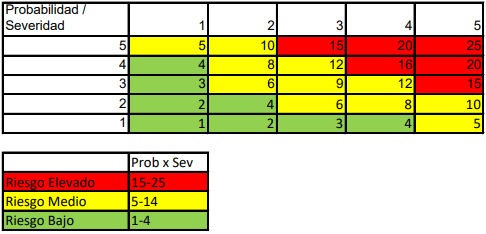
\includegraphics[width=0.8\textwidth]{./images/risk-definition.jpg}
    \caption{Planilla de Definicion de Riesgos}
    \label{fig:rd}
\end{figure}

\begin{figure}[ht]
    \centering
    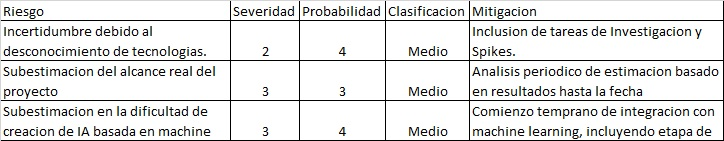
\includegraphics[width=0.8\textwidth]{./images/risk-management.jpg}
    \caption{Planilla de Control de Riesgos}
    \label{fig:rc}
\end{figure}


\end{document}

